\chapter{Návrh}
\label{kap:nav}
V tejto kapitole sa budeme zaoberať návrhom jednotlivých častí aplikácie. Najskôr spomenieme funkcie, ktoré bude naša aplikácia ponúkať. Ďalej popíšeme, ako sme spomedzi mnohých alternatív vybrali vhodný algoritmus pre potrebu našej aplikácie. Pri navrhovaní aplikácie sme sa venovali analýze získaných statických dát a dát o meškaní. Uvádzame tiež, ako budeme pristupovať k týmto dátam pri implementácii. V neposlednom rade spomenieme, ako bude fungovať naša aplikácia z pohľadu jej architektúry.

\section{Funkcie aplikácie}
Ako sme si mohli všimnúť v \ref{sec:applications}, všetky aplikácie ponúkajú vyhľadávanie z aktuálnej polohy rovnako ako aj možnosť výberu zastávky priamo z mapy. Tieto funkcie bude používateľovi ponúkať aj naša aplikácia. Väčšina spomenutých aplikácií ponúkala zobrazenie histórie vyhľadávania, ktorá odľahčí používateľa od zadávania parametrov v prípade, že vyhľadáva väčšinou tie isté spoje. Túto funkcionalitu nájde používateľ aj v našej aplikácii. História vyhľadávania sa bude ukladať do pamäte zariadenia. 

Vo väčšine aplikácií si používatelia vedia zobraziť všetky linky v MHD a postupnosti zastávok, ktoré obsluhujú. Túto funkciu bude ponúkať aj naša aplikácia. Čo sa týka nastavenia prídavných preferencií pri vyhľadávaní, aplikácie ponúkajú rôzne preferencie. Najčastejšími z nich sú: maximálny počet prestupov, minimálny čas na prestup, limit pre peší presun a zobrazenie len nízkopodlažých vozidiel. Naša aplikácia bude mať možnosť nastavenia všetkých týchto preferencií.

Jediná aplikácia, ktorá ponúka informácie o reálnom pohybe vozidiel vo forme meškania, je aplikácia \textit{UBIAN}. Predpokladáme však, že aj táto aplikácia vyhľadáva v statických cestovných poriadkoch a pri vyhľadanom spoji len pripíše informáciu vo forme meškania. Uvažujeme tak na základe toho, že po vyhľadaní spojov zo zastávky po zadaní aktuálneho času aplikácia ponúkne také spoje, ktoré podľa statických cestovných poriadkov majú na túto zastávku v blízkej budúcnosti príchod. Ak existuje taký spoj, ktorý mal odchod z danej zastávky v minulosti, ale má meškanie a na zastávke ešte nebol, aplikácia ho nezobrazí. Naša aplikácia ponúkne aj tie spojenia, ktoré kvôli meškaniu na zastávku ešte nedorazili.

Medzi ďalšie funkcionality patrí zakúpenie lístka priamo prostredníctvom aplikácie. Táto funkcionalita však nesúvisí priamo so zadaním našej práce a navyše je potrebná zmluva s dopravcami. Preto naša aplikácia túto možnosť ponúkať nebude.

Jediná aplikácia, ktorá dokáže vyhľadávať cesty aj v offline režime je \textit{CG Tranzit}. Hoci je užitočné ponúknuť vyhľadávanie bez možnosti prístupu na internet, znamenalo by to, že náš algoritmus by bežal na klientskej strane.  Keďže hlavnou úlohou našej aplikácie je vyhľadávanie spojov z reálnych dát, aplikácia bude fungovať online s tým, že zaručí používateľom vždy aktuálne spojenia. 

V tabuľke \ref{table:aplication-funcions} je zobrazený prehľad funkcionalít našej navrhovanej aplikácie a iných existujúcich aplikácii na vyhľadávanie spojov v MHD Bratislava.

\begin{table}[H]
\footnotesize
\begin{tabular}{|L{4.49cm}|c|c|c|C{1.29cm}|c|C{1.54cm}|}
\hline
\rowcolor[HTML]{C0C0C0} 
\textbf{} & \textbf{Imhd.sk} & \textbf{IDS BK} & \textbf{CP} & \textbf{CG Tranzit} & \textbf{UBIAN} & \textbf{Naša aplikácia}
\\ \hline
\textbf{z aktuálnej polohy} & \cmark & \cmark  & \cmark  & \cmark  & \cmark  & \cmark    
\\ \hline
\textbf{výber zástavok z mapy} & \cmark & \cmark  & \cmark  & \cmark  & \cmark & \cmark       
\\ \hline
\textbf{história vyhľadávania} & \cmark & \xmark  & \cmark  & \cmark  & \cmark & \cmark         
\\ \hline
\textbf{zobrazenie liniek} & \cmark & \cmark  & \xmark  & \cmark  & \xmark & \cmark         
\\ \hline
\textbf{max. počet prestupov} & \cmark & \cmark  & \cmark  & \cmark  & \xmark & \cmark         
\\ \hline
\textbf{min. čas na prestup} & \cmark & \xmark  & \cmark  & \cmark  & \xmark & \cmark         
\\ \hline
\textbf{limit pre peší presun} & \cmark & \cmark  & \xmark  & \xmark  & \xmark  & \cmark        
\\ \hline
\textbf{len nízkopodlažné vozidlá} & \cmark & \xmark  & \cmark  & \xmark  & \xmark  & \cmark        
\\ \hline
\textbf{meškanie MHD} & \xmark & \xmark  & \xmark  & \xmark  & \cmark & \cmark         
\\ \hline
\textbf{kúpa lístkov} & \xmark & \cmark  & \cmark  & \cmark  & \cmark & \xmark         
\\ \hline
\textbf{offline režim} & \xmark & \xmark  & \xmark  & \cmark  & \xmark  & \xmark        
\\ \hline
\end{tabular}
\caption{Tabuľka funkcionalít existujúcich aplikácií a navrhovanej aplikácie}
\label{table:aplication-funcions}
\end{table}

\section{Dáta}
Pri vývoji aplikácie a pre jej testovanie sú nevyhnutné dáta. Pre účely aplikácie budeme potrebovať dáta zo statických cestovných poriadkov a dáta o meškaní jednotlivých jázd. 

\subsection{Dáta statických cestovných poriadkov}
Od Dopravného podniku Bratislava sme získali statické cestovné poriadky, ktoré mali platnosť od $5.2.2018$ – $31.12.2018$. Dáta sú vo formáte GTFS. 

\subsubsection{GTFS}
\label{sec:gtfs}
\textit{General Transit Feed Specification (GTFS)} je dohodnutý formát dát, ktorý používajú tisíce poskytovateľov verejnej dopravy a mnohé softvérové aplikácie. Špecifikácia definuje súbory, v ktorých sú reprezentované entity v tabuľke. V stĺpcoch sú popísané vlastnosti entity a v každom riadku je nový záznam. V tejto sekcii analyzujeme len tie súbory, ktoré nám boli poskytnuté a opíšeme, ktoré z poskytnutých údajov využijeme.

Súbor \textit{agency.txt} obsahuje údaje o prepravných spoločnostiach. Tento súbor nebudeme potrebovať, kedže všetky linky spravuje jedna spoločnosť. 

Súbor \textit{calendar.txt} obsahuje stĺpce \textit{service\_id}, \textit{monday}, \textit{tuesday}, \textit{wednesday}, \textit{thursday}, \textit{friday}, \textit{saturday}, \textit{sunday}, \textit{start\_date}, \textit{end\_date}. Vlasntosť \textit{service\_id} predstavuje unikátny názov typu dňa (pracovný deň, víkend,...). Vlasnosti \textit{monday, ..., sunday} môžu nadobúdať hodnoty $0$ a $1$. Ak je napríklad hodnota $monday = 1$, znamená to, že všetky pondelky medzi dátumom \textit{start\_date} a dátumom \textit{end\_date} patria do typu dňa \textit{service\_id}. Naopak, ak je hodnota rovná $0$, tak nepatria. 

V súbore \textit{calendar\_dates.txt} sú vlastnosti: \textit{service\_id}, \textit{date}, \textit{exception\_type}. V prípade, že vlastnosť \textit{exception\_type} má hodnotu $1$, znamená to, že do \textit{service\_id} výnimočne patrí aj deň \textit{date}. Ak je $exception\_type = 2$, tak nepatrí.

Zastávky sú definované v súbore \textit{stops.txt}. Zastávka je určená identifikačným číslom \textit{stop\_id}, ktoré je unikátne pre každú zastávku. Identifikačné číslo zastávky obsahuje na začiatku viac núl, ktoré môžeme odignorovať. Vlastnosť \textit{stop\_name} predstavuje názov zastávky. Táto vlastnosť sa nachádza v súbore viackrát, kedže v rámci zastávky existujú rôzne nástupištia. Unikátnymi vlastnosťami sú aj \textit{stop\_lat} a \textit{stop\_lng}, teda súradnice zastávky. Zastávka má definovanú aj \textit{zone\_id}, teda zónu mesta, do ktorej je zastávka priradená. Jednotlivé stĺpce sú v súbore oddelené čiarkou, avšak čiarka sa môže nachádzať aj v názve zastávky. V takom prípade je názov zastávky uvedený v úvodzovkách.

Súbor \textit{routes.txt} obsahuje zoznam liniek. Pre každú linku definuje identifikačné číslo linky (\textit{route\_id}), číslo prepravnej spoločnosti (\textit{agency\_id}), skrátený názov linky (\textit{route\_short\_name}) a mód linky (\textit{route\_type}). Podľa štandardu \textit{GTFS} hodnota $0$ definuje mód električku, hodnota $3$ predstavuje autobus a hodnota $11$ trolejbus. Vlastnosť \textit{route\_long\_name} nie je definovaná a vlastnosť \textit{route\_text\_color} pre nás nie je potrebná.

Jazdy jednotlivých liniek sú zaznamenané v súbore \textit{trips.txt}, ktorý obsahuje vlastnosti: identifikačné číslo jazdy (\textit{trip\_id}), \textit{service\_id}, \textit{trip\_headsign}, \textit{trip\_short\_name} a \textit{direction\_id}. Podľa GTFS špecifikácie by vlastnosť \textit{service\_id} mala predstavovať množinu rôznych \textit{service\_id} oddelených pomlčkou. V našich dátach existuje pre jeden záznam jazdy len jeden \textit{service\_id}. Vlastnosť \textit{trip\_headsign} predstavuje konečnú zastávku jazdy. Túto vlastnosť síce nevyužijeme, ale kedže obsahuje názvy zastávok rovnako ako v súbore \textit{stops.txt}, môže sa stať, že názov bude obsahovať oddelovač stĺpcov - čiarku. Vlastnosť \textit{trip\_short\_name} nie je definovaná v žiadnom zázname jazdy. \textit{Direction\_id} nadobúda hodnoty $0$ a $1$. V dátach nám chýba informácia o nízkopodlažných spojoch, ktorú sme chceli využiť pri vyfiltrovaní hľadaných ciest.

Súbor \textit{stop\_times.txt} definuje indentifikačné číslo jazdy (\textit{trip\_id}), identifikačné číslo zastávky (\textit{stop\_id}), čas príchodu a odchodu jazdy na zastávku (\textit{arrival\_time} a \textit{departure\_time}), \textit{stop\_sequence}, \textit{stop\_headsign}, \textit{pickup\_type} a \textit{drop\_off\_type}. Vlastnosti \textit{arrival\_time} a \textit{departure\_time} sú vždy rovnaké, preto jednu z nich budeme ignorovať. Vlastnosť \textit{stop\_sequence} predstavuje poradie zastávky v rámci linky. Poradie nie je iterované od $1$, ale začína rôznymi kladnými číslami. Položka \textit{stop\_headsign} nie je v žiadnom zázname definovaná. Vlastnosti \textit{pickup\_type} a \textit{drop\_off\_type} nadobúdajú hodnoty $0$ a $3$. V \textit{GTFS} špecifikácii znamená číslo $0$, že jazda na tejto zastávke stojí vždy a $3$ určuje, že jazda na zastávke stojí len na znamenie. Hodnoty sú pre obe vlastnosti vždy rovnaké, takže jednu z nich môžeme opäť ignorovať.


\subsection{Dáta o meškaní}
\label{sec:delay-data}
Dopravný podnik Bratislava nám poskytol aj informácie o meškaní za rok 2018, pre mesiac február, marec a apríl. Pre každý deň v mesiaci existuje súbor vo formáte \textit{csv}. Každý záznam obsahuje údaje: identifikačné číslo záznamu, dátum a čas, kedy bol záznam o meškaní zaevidovaný, identifikačné číslo vozidla, názov linky, poradie, číslo zastávky, názov zastávky a meškanie.

Z pozorovania dát vyplýva, že vlastnosť hodnota meškania nadobúda hodnotu $0$, kladné a záporné celé čísla alebo hodnotu $n/a$. Na prelome dní sa v dátach vyskytuje hodnota meškania $-1229$, ktorú budeme ignorovať. Riadky, ktoré majú hodnotu meškania $n/a$ budeme tiež ignorovať.

Aby sme boli schopní správne zohľadniť meškanie v našom algoritme, potrebujeme hodnotu meškania zapísať do dátovej štruktúry. Na to potrebujeme vedieť identifikačné číslo zástavky a konkrétnu jazdu linky, na ktorej meškanie vzniklo. 

Z poskytnutých dát vieme zistiť číslo zastávky, ktoré sa však nezhoduje s identifikačnými číslami zastávok získaných z dát statických cestovných poriadkov. Po menšej analýze sme zistili, že poskytnuté čísla zastávok sa podobajú na tie identifikačné. Ak sa vyskytuje v čísle zastávky nula, tak k nule, ktorá je najviac vpravo pridáme ďalšie tri nuly. Týmto získame identifikačné číslo zastávky.

Ďalej potrebujeme vedieť priradiť poskytnutý názov linky ku konkrétnej linke zo statických dát. Názov linky je v statických dátach unikátny, takže linku môžeme vyhľadať aj podľa názvu. V dátach o meškaní existujú také názvy liniek, ktoré sa nenachádzajú v tých statických. Sú to napríklad trojciferné čísla začínajúce cifrou $4$. Ak cifru $4$ zmeníme na písmeno $N$, názvy liniek sa zhodujú s názvami nočných spojov. Existujú aj ďalšie názvy liniek, ktoré nenájdeme v zozname liniek statických cestovných poriadkov. Tieto už budeme ignorovať. 

Pôvodne sme si mysleli, že údaj poradie určuje poradie jazdy v rámci linky. Nie je to však tak, keďže hodnoty sú príliš malé. Máme však už všetky údaje potrebné na špecifikovanie správnej jazdy. Poznáme identifikačné číslo linky $r$, poznáme hodnotu meškania $d$ jazdy $t$ na zastávku $p$ a poznáme aj čas a dátum $\tau$, kedy boli tieto údaje zaznamenané. Po pripočítaní $d$ minút k času $\tau$, získame približný čas, kedy stojí hľadaná jazda $t$ linky $r$ na zastávke $p$. Neexistujú dve jazdy jednej linky, ktoré stoja na zastávke v rovnakom čase v rovnaký typ dňa. Týmto spôsobom získame jazdu, ktorej meškanie prislúcha.

Získané dáta umožňujú našej aplikácii ponúknuť správne cesty s prihliadnutím na meškanie spojov od $5.2.2018$ – $30.4.2018$. Statické vyhľadávanie bez meškania bude správne fungovať od $5.2.2018$ do konca roka $2018$.


\subsection{Pešie presuny}
\label{sec:foot-paths}
V dátach sa nenachádzajú informácie o peších presunoch. V sekcii \ref{sec:raptor-improved} bolo navrhnuté, ako vypočítať peší presun s použitím Manhattanovskej vzdialenosti, prípadne penalizovať prestupy podľa ich typu. Napokon sme sa rozhodli využiť   \textit{Google API}, ktoré okrem iného ponúka možnosť vyhľadania peších vzdialeností medzi 2 bodmi prostredníctvom \textit{Distance Matrix API}. Počet bezplatných dopytov na \textit{Distance Matrix API} je však obmedzený. Z toho dôvodu nebudeme vyhľadávať pešie presuny pri hľadaní cesty. Vytvoríme jednorazovo súbor \textit{foot\_paths.txt}, ktorý bude obsahovať údaje o peších presunoch, ktoré sú pre nás zaujímavé. Nebudeme vyhľadávať pešie vzdialenosti medzi každou dvojicou zastávok, nakoľko to nie je potrebné. 

Budeme postupovať nasledovne: pre každú zastávku $p$ nájdeme zastávky v okolí 800 metrov radiálnym vyhľadávaním. Pomocou \textit{Distance Matrix API} zistíme vzdialenosti nájdených zastávok od zastávky $p$. Každú dvojicu zastávok uložíme do súboru spolu so zistenými vzdialenosťami určenými v minútach.

\section{Databáza}

Na serveri budú uložené dáta aplikácie v PostgreSQL databáze. Databáza sa naplní pri prvotnom spustení aplikácie na serveri. Schéma databázy je popísaná entitno-relačným diagramom na obrázku \ref{fig:erd}.

\begin{figure}[H]
\centerline{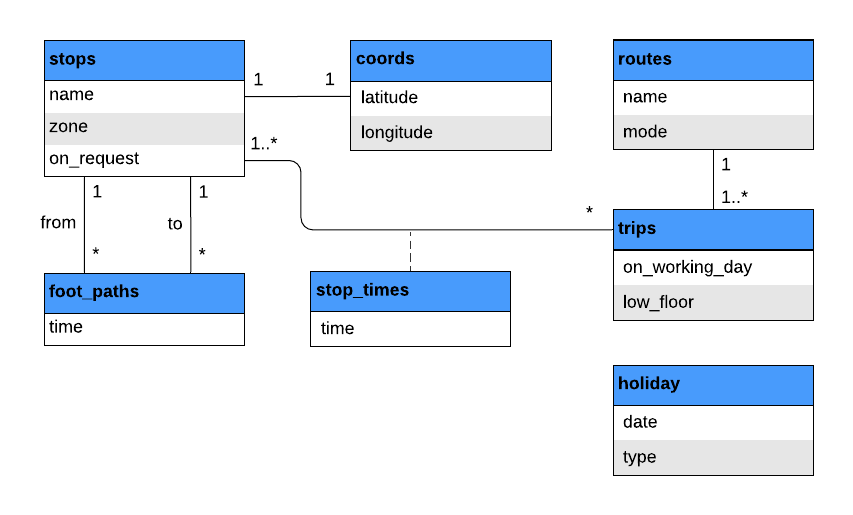
\includegraphics[width=1.0\textwidth]{images/ERD}}
\caption[Entitno-relačný diagram]{Entitno-relačný diagram}
\label{fig:erd}
\end{figure}

Entita \textit{stop\_areas} obsahuje zoskupenie zastávok, ktoré majú rovnaké názvy (\textit{name}). 


V entite \textit{stops} evidujeme zónu mesta (\textit{zone}), do ktorej zastávka patrí. Hodnota \textit{on\_request} určuje, či sa na  zastávke nastupuje a vystupuje na znamenie. Každá zastávka má priradené súradnice, ktoré sa udržujú v entite \textit{coords}.

V entite \textit{coords} sú súradnice určené atribútmi zemepisná šírka (\textit{latitude}) a zemepisná výška (\textit{longitude}). 

Entita \textit{foot\_paths} obsahuje atribút \textit{time}, ktorý určuje čas v minútach potrebný na peší presun zo zastávky \textit{from} na zastávku \textit{to}.

V entite \textit{routes} sa udržuje zoznam liniek jazdiacich v bratislavskej MHD. Linka je určená názvom (\textit{name}) a módom (\textit{mode}). V Bratislave jazdia 3 rôzne módy: električka, trolejbus a autobus. Každá linka má počas dňa viaceré jazdy (\textit{trips}).

Entita (\textit{trips}) uchováva informáciu o tom, či je vozidlo, ktoré bolo pridelené konkrétnej jazde nízkopodlažné (\textit{low\_floor}), ktorým smerom ide (\textit{direction}) a zároveň počas akých typov dní (\textit{service\_day}) jazda premáva. Každá jazda linky je tvorená postupnosťou zastávok, ktoré linka obsluhuje.

V entite \textit{stop\_times} je zachytený čas (\textit{time}), kedy jazda stojí na zastávke a v akom poradí sú zastávky v rámci jazdy (\textit{sequence\_order}).

V entite \textit{service\_days} sú názvy rôznych typov dní, v ktorých premávajú jazdy liniek. 

Entita \textit{calendar\_dates} obsahuje zoznam všetkých dátumov (\textit{date}) v rozsahu platnosti cestovného poriadku. Ku každému dátumu je priradený typ dňa (\textit{service\_day}). Jeden dátum môže prislúchať k viacerým typom dňa a naopak jeden typ dňa môže prislúchať viacerým dátumom.


\section{Parametre pre algoritmus}
Používateľ môže pre vyhľadanie ciest zadať začiatočnú a konečnú zastávku tak, že vyberie zastávky z ponúkaného zoznamu zastávok. V zozname predstavuje zastávka \textit{stop area}, ktorá zoskupuje zastávky s rovnakým názvom a rôznymi identifikačnými číslami. Preto vyhľadávanie ciest medzi začiatočnou a konečnou zastávkou bude vyhľadávanie ciest medzi  dvomi množinami zastávok, ako je ilustrované na obrázku \ref{fig:initial-parameters} a).

\subsubsection{Vyhľadávanie z aktuálnej polohy}
Začiatočný bod vie používateľ vybrať aj ako aktuálnu polohu, na ktorej sa nachádza. Radiálnym vyhľadávaním nájdeme okolité zastávky, ako bolo spomenuté v \ref{sec:actual-location}. Najbližšia vyhľadaná zastávka k aktuálnemu bodu nemusí znamenať optimálne riešenie a preto budeme považovať za začiatočnú zastávku každú z nich. Pre každú z týchto zastávok zistíme vzdialenosť od aktuálnej polohy  v minútach použitím \textit{Distance Matrix API}. 

Tieto zastávky vytvoria množinu začiatočných zastávok s informáciou o iniciálnych vzdialenostiach z aktuálnej polohy do začiatočnej zastávky. Tento prípad je zobrazený na obrázku \ref{fig:initial-parameters} b). Do finálneho riešenia zakomponujeme peší presun od aktuálnej polohy po začiatočnú zastávku vybraných optimálnych ciest. Pri vstupných parametroch bude informácia o tom, či používateľ vyhľadával z aktuálnej polohy.

\begin{figure}[H]
\centerline{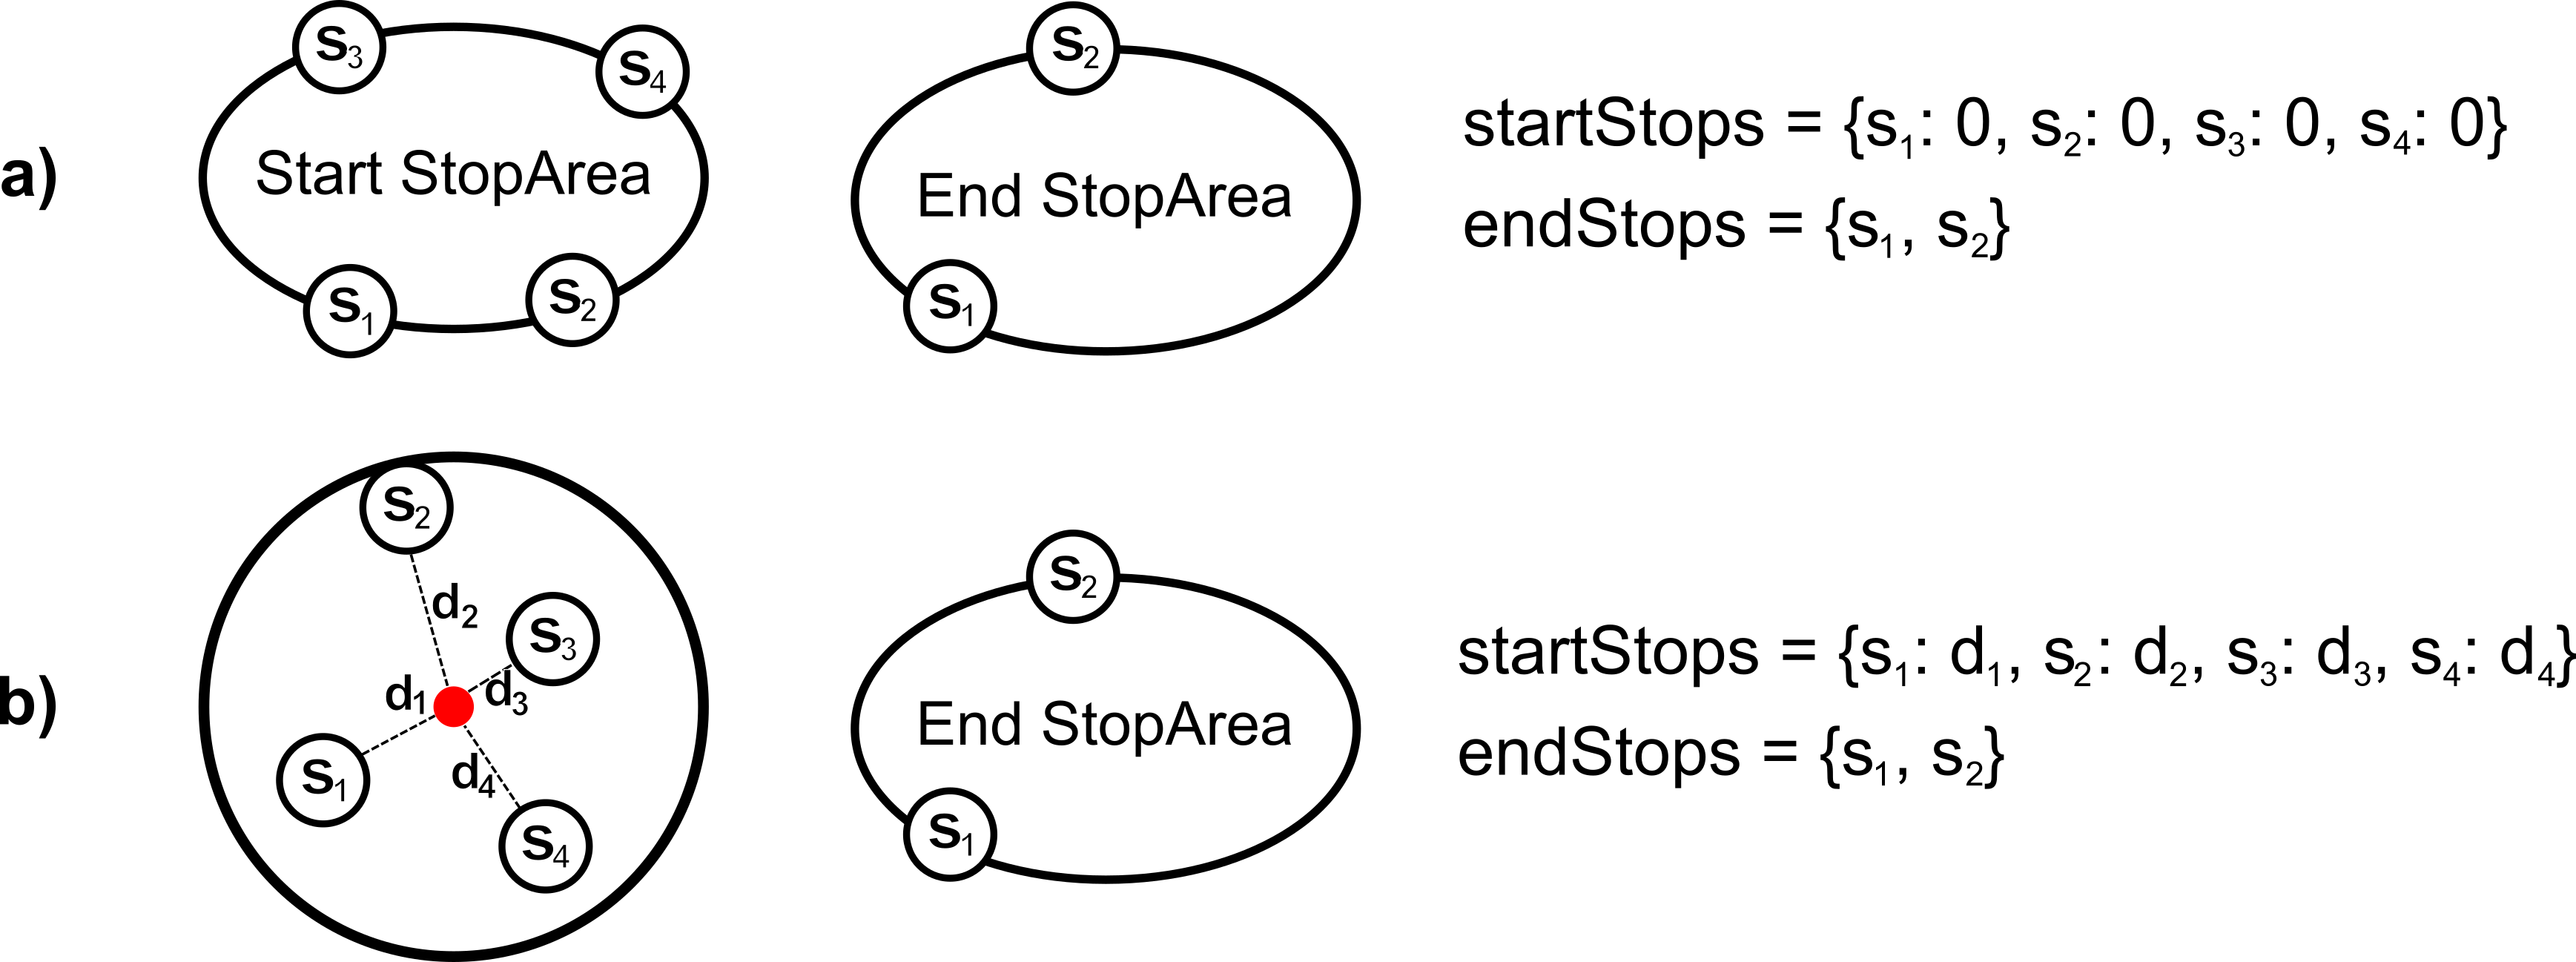
\includegraphics[width=1.0\textwidth]{images/initial-parameters}}
\caption[Vstupné množiny zastávok]{Vstupné množiny zastávok}
\label{fig:initial-parameters}
\end{figure} 

Vstupom pre algoritmus bude teda množina začiatočných zastávok aj s iniciálnymi vzdialenosťami. V prípade, že nevyhľadávame z aktuálnej polohy, budú mať vzdialenosti hodnotu 0. Vstup algoritmu tvorí aj množina konečných zastávok, dátum a čas, 4 parametre predstavujúce používateľské preferencie a informácia o vyhľadávaní z aktuálnej polohy.

\section{Algoritmus}
Pri hľadaní algoritmu na nájdenie optimálnej cesty sme najskôr siahli po najznámejšom vyhľadávacom grafovom algoritme. Dijkstrov algoritmus \ref{sec:dijkstra} sa zdal vhodný, avšak jeho vylepšená verzia A* algoritmus \ref{sec:a-star} je pri správne zvolenej heuristike efektívnejšia. Keďže zastávky, ktoré predstavujú vrcholy v grafe majú dané súradnice, uvažovali sme aj o optimalizovaní prehľadávaného priestoru. Pri štúdiu článkov sme narazili na rôzne optimalizácie prehľadávaného priestoru. Minimalizácia v okolí virtuálnej cesty a minimalizácia \textit{bounding boxom} sú spomenuté v \ref{sec:optimalization}.

V prípade cestovných poriadkov je náročné správne namodelovať graf, ktorý dokáže efektívne spracovať časovo závislé dáta. V \ref{sec:models} boli spomenuté dva overené prístupy \textit{Time dependent} a \textit{Time expanded model}, ktoré tento problém riešia. 

Ďalšou výzvou je prispôsobiť grafový vyhľadávací algoritmus, aby dokázal vypočítať alternatívne optimálne cesty, prihliadal na prestupy medzi rôznymi módmi a popri tom počítal s ďalšími pridanými kritériami.
V \ref{sec:time-dependant-algorithm} boli spomenuté návrhy časovo závislých algoritmov, ktoré niektoré z týchto problémov riešia. Algoritmus v \ref{sec:multimodal-algorithm} sa dokáže vysporiadať aj viacerými módmi. Vráti však len jednu cestu. Na hľadanie alternatívnych ciest, by sme mohli použiť algoritmus spomenutý v \ref{sec:alternative-optimal-paths}.

Kvôli dynamickej povahe verejnej dopravy grafový prístup v kombinácii s vyhľadávacím grafovým algoritmom vyžaduje veľa pre-processingu a to sa odráža na výpočtových časoch. Výhodou vo verejnej doprave je, že vozidlá sa pohybujú po vyznačených linkách, ktorých trasy poznáme. Schéma verejnej dopravy sa preto dá zachytiť do pomerne jednoduchých dátových štruktúr. Tento fakt si všimli aj autori algoritmu RAPTOR, ktorý sme opísali v \ref{sec:raptor}. 

V našej aplikácii sme sa rozhodli použiť tento negrafový algoritmus. Jeho výhodou je, že nie je potrebné vytvárať model a nie je potrebné osobitne riešiť multimodalitu hromadnej dopravy. Ľahšie zvláda dynamickosť dát ako meškanie linky, zrušenie linky alebo zmenu trasy. 

\subsection{Použitie a prispôsobenie RAPTOR algoritmu}
RAPTOR algoritmus počíta s tým, že každá linka pozostáva z jázd, ktoré majú rovnaké postupnosti zastávok, ako bolo spomenuté v \ref{sec:raptor-definitions}. Pri skúmaní dát sme zistili, že v prípade našich dát táto vlastnosť nie je splnená. Bude potrebné prispôsobiť algoritmus aj dátovú štruktúru, aby zohľadňovali rôzne postupnosti zastávok v rámci linky.

\subsubsection{Optimalizácia}
Na základnú verziu RAPTOR algoritmu popísanú v \ref{sub:raptor-basic} použijeme aj jeho optimalizáciu opísanú v \ref{sub:raptor-optimalisation}, kedy označujeme zastávky, aby sme nemuseli prechádzať tie linky, ktorým sa nevylepšil čas $\tau_{k-1}(p)$. Označené zastávky predstavujú potenciálne prestupné zastávky.  Rovnako využijeme aj optimalizácie \textit{local-prunning} a \textit{target-prunning}, ktoré nám zredukujú počet označených zastávok. Pri optimalizácii \textit{target-prunning} však nebudeme využívať hodnotu $\tau^*(p_t)$, ktorá predstavuje najlepší čas do konečnej zastávky $p_t$. Nás zaujíma čas $\tau^*(P_t)$, ktorý predstavuje najlepší čas zo všetkých zastávok zoskupených v konečnej \textit{stop area} $P_t$. 

\subsubsection{Zapracovanie dát o meškaní}
Kedže cieľom našej práce je vyhľadávanie ciest s prihliadnutím na prípadné meškania spojov, potrebujeme dosiahnuť, aby algoritmus pri hľadaní optimálnych ciest prihliadal na zaznamenané meškania. Spoliehame sa na to, že dátová štruktúra si bude držať pri každej zastávke v každej jazde hodnotu meškania. Prihliadať na meškania budeme len v prípade, že používateľ vyhľadáva v aktuálny deň. Inak bude údaje o meškaniach ignorovať a vyhľadávať cesty zo statických cestovných poriadkov.

\subsubsection{Preferencie}
Okrem základných povinných vstupných parametrov ponúkame používateľovi možnosť zvoliť si prídavné parametre vyhľadávania. Okrem začiatočnej a konečnej zastávky, času a dátumu vyhľadávania si bude môcť používateľ zvoliť aj maximálny počet prestupov, maximálnu dĺžku pešieho presunu v minútach, ako aj minimálny čas na prestup medzi dvoma linkami. Používatelia s hendikepom, kočíkom alebo bicyklom budú môcť vyhľadávať len nízkopodlažné spoje. Ďalším vylepšením algoritmu teda je, že algoritmus bude zohľadňovať všetky tieto používateľské kritériá. 

\subsubsection{Alternatívne cesty}
Po dobehnutí RAPTOR algoritmu získame tabuľku najlepších časov pre každé kolo a každú zastávku. Pod najlepším časom v kole $k$ pre zastávku $p$ rozumieme najskorší možný čas, ktorým sa vieme dostať na zastávku $p$ na $k-1$ prestupov. Keďže používame optimalizáciu \textit{local-prunning}, máme pre každú zastávku evidovaný čas $\tau^*(p)$, ktorý predstavuje celkovo najlepší čas pre zastávku $p$ bez ohľadu na počet prestupov. Našim cieľom však nie je získať jednu najkratšiu cestu, ale alternatívne optimálne cesty.

V sekcii \ref{sec:raptor-improved} sme spomenuli vylepšený RAPTOR algoritmus, ktorý pre každú zastávku nehľadá najlepší čas, ale $K$ optimálnych ciest. Prihliada na to, aby cesty neboli podobné na veľkej časti úsekov. Po dobehnutí algoritmu máme pre každú zastávku najviac $K$ optimálnych ciest.

Najskôr sme použili spomínané navrhnuté vylepšenie RAPTOR algoritmu, narážali sme však na problém, ako správne zvoliť premennú $K$, aby sme neodfiltrovali tie cesty, ktoré môžu byť správne. Navyše po každom vylepšení času $\tau^*_k(p)$ bolo potrebné prejsť všetky cesty v množine $\mathcal{J}_k(p)$ a odfiltrovať najmenej efektívne. Cesty by boli vyfiltrované len v rámci zastávok (\textit{stop}) a nie pre celú skupinu zastávok (\textit{stopArea}).

Rozhodli sme sa napokon využiť základnú verziu algoritmu, kedy získavame tabuľku najlepších časov. Budeme si pamätať, ako sme dosiahli každý z vylepšených časov. Budeme evidovať, z ktorej zastávky sme sa na označenú zastávku dostali a akým spôsobom. Z výsledkov vytvoríme len také cesty, ktoré končia v niektorej z konečných zastávok a začínajú v niektorej zo začiatočných zastávok. Tieto cesty budeme filtrovať podľa potrebných filtrov, aby sme získali cesty, ktoré sú optimálne. 

\subsubsection{Filtre}
Všetky cesty, ktoré budú výsledkom dopytu, musia vyhovovať nasledujúcim filtrom. RAPTOR algoritmus operuje v kolách a v každom kole hľadá zastávky, ktorým vieme vylepšiť čas. Tieto zastávky dosahuje akciami. Každá akcia začína v niektorej z označených zastávok $p_m$ v kole $k-1$ a končí v inej dosiahnuteľnej zastávke $p_i$ v kole $k$.  Ako sme už spomínali zastávka $p_m$ je prestupné miesto. Pod akciou teda rozumieme buď peší presun zo zastávky $p_m$ do zastávky $p_i$ alebo úsek jazdy pričom platí, že $p_m$ je zastávka na nastúpenie a zastávka $p_i$ je zastávka na vystúpenie.

Cesta je vlastne postupnosťou zastávok $(p_0, p_1, …, p_n)$ a akcií $(a_0, a_1, ..., a_{n-1})$. Nechceme povoliť, aby v rámci cesty boli obe akcie $p_i, p_{i+1}$ akciami pešieho presunu. V súčte by časy trvania po sebe nasledujúcich peších presunov mohli prekročiť maximálne zadané trvanie pešieho presunu. 

Ďalej nechceme povoliť, aby zastávka $p_0$ a $p_1$ patrili do rovnakej \textit{stop area}. Toto obmedzenie platí aj pre zastávky $p_{n-1}$ a $p_n$.

Ďalej filtrujeme cesty ich porovnávaním medzi sebou navzájom. Majme cesty, ktoré už prešli cez všetky vyššie spomínané kritériá. Nech cesta $J_1$ začína v čase $dt_1$, končí v čase $at_1$ a obsahuje $m$ prestupov. Nech cesta $J_2$ má začiatočný čas $dt_2$, konečný čas $at_2$ a obsahuje $n$ prestupov. V sekcii \ref{sec:raptor-improved} boli okrem iného spomenuté aj podobné cesty. Problém podobných ciest sme ilustrovali na obrázku \ref{fig:similar-paths}. V prípade že platí $dt_1 = dt_2, at_1=at_2$ a $m < n$, tak cestu $J_2$ chceme odfiltrovať. V inom prípade nech platí, že $dt_1 = dt_2, at_1=at_2$ a $m=n$ a zároveň platí, že jednotlivé úseky jázd patria rovnakej linke, tak odfiltrujeme jednu z nich. Tieto cesty sa líšia len prestupným miestom. 

Chceme filtrovať nevýhodné cesty. Nech platí $dt_1 \leq dt_2$ a $ar_1 > ar_2$, tak cestu $J_1$ odfiltrujeme. Rovnako aj keď platí $dt_1 < dt_2$ a $ar_1 \geq ar_2$ chceme cestu $J_1$ odfiltrovať. 

Dostávame sa ešte k takým cestám, pre ktoré platí $dt_1 \leq dt_2, at_1<at_2$ a $m>n$. Cestujúcich môže zaujímať aj cesta $J_2$, ktorou sa síce nedostaneme do konečnej zastávky najrýchlejšie, ale obsahuje menší počet prestupov ako cesta $J_1$. Otázkou je s akým omeškaním času príchodu je cesta $J_2$ ešte prijateľná. Rozhodli sme sa prestup penalizovať $x$ minútami. Nech platí, že cesta $J_1$ je cesta, ktorou sa dostaneme najskôr do konečnej zastávky a nech $(at_2-at_1) > (m-n) * x$, tak cestu $J_2$ odfiltrujeme.

\subsubsection{Nasledujúce cesty}
Takto vylepšený algoritmus nájde niekoľko optimálnych ciest najskôr od hľadaného času a dátumu. My však chceme používateľovi zobraziť určitý počet ciest na jednu podstránku a teda potrebujeme vyhľadané cesty doplniť nasledujúcimi cestami. 
Riešením tohto problému by mohol byť rRAPTOR algoritmus spomínaný v 1.8.4. Takto vylepšený algoritmus však nepočíta s tým, že cesta môže začínať peším presunom. Budeme preto používať iný mechanizmus hľadania nasledujúcich ciest.
Zvolíme si konštantu $x$, ktorá predstavuje minimálny počet ciest na podstránke. Keď vyhľadáme cesty po čase $\tau$, algoritmus nájde $k$ optimálnych ciest, pričom začiatočný čas poslednej ciest je $t$. Ďalšie vyhľadávanie spustíme s časom $t + 1$ minúta. Vyhľadané cesty pridáme k predchádzajúcim a na tieto cesty aplikujeme ešte niektoré z filtrov. Takto budeme pokračovať, kým nemáme vyhľadaných aspoň $x$ ciest.

\subsubsection{Zhrnutie}
Výstupom z nášho algoritmu bude množina aspoň $x$ ciest začínajúcich na niektorej zastávke $p_s$ zo skupiny ciest $P_s$, po čase $\tau$ a končiacich v niektorej zastávke $p_t$ zo skupiny ciest $P_t$. Jednotlivé cesty sú optimálne, nie sú si podobné na väčšine úsekov a vyhovujú prípadným používateľským preferenciám.

\section{Dátová štruktúra}
Aby algoritmus dokázal rýchlo nájsť optimálne cesty, potrebuje efektívne navrhnutú dátovú štruktúru. Pri jej návrhu sme sa inšpirovali dátovou štruktúrou z \ref{subsec:structure}, ktorá bola navrhnutá pre základnú verziu RAPTOR algoritmu. Dátová štruktúra uvedená v článku počíta so skutočnosťou, že jednotlivé jazdy v rámci linky majú rovnakú postupnosť zastávok. Avšak v našich dátach to tak nie je. 

Linky v našich dátach obsahujú jazdy, ktoré idú jedným aj druhým smerom. Zastávky, cez ktoré prechádza linka majú síce rovnaký názov, ale majú iné identifikačné čísla, ktorými sú definované a hlavne ich postupnosť je iná. Okrem rôznych smerov obsahuje linka aj také jazdy, ktorých postupnosť zastávok je iná ako pri väčšine. Najmä v ranných a večerných hodinách prechádzajú niektoré jazdy len cez určitú podpostupnosť zastávok. 

RAPTOR algoritmus potrebuje, aby všetky jazdy, ktoré patria konkrétnej linke mali rovnakú postupnosť zastávok. Rozhodli sme sa preto zoskupiť jazdy linky s rovnakou postupnosťou zastávok do úsekov linky (\textit{subroutes}). Teraz platí, že 1 linka (\textit{route}) má viacero úsekov a jednému úseku linky prislúcha viac jázd linky (\textit{trips}). Upravená štruktúra je zachytaná na obrázku \ref{fig:my-datastructure}.

\begin{figure}[H]
\centerline{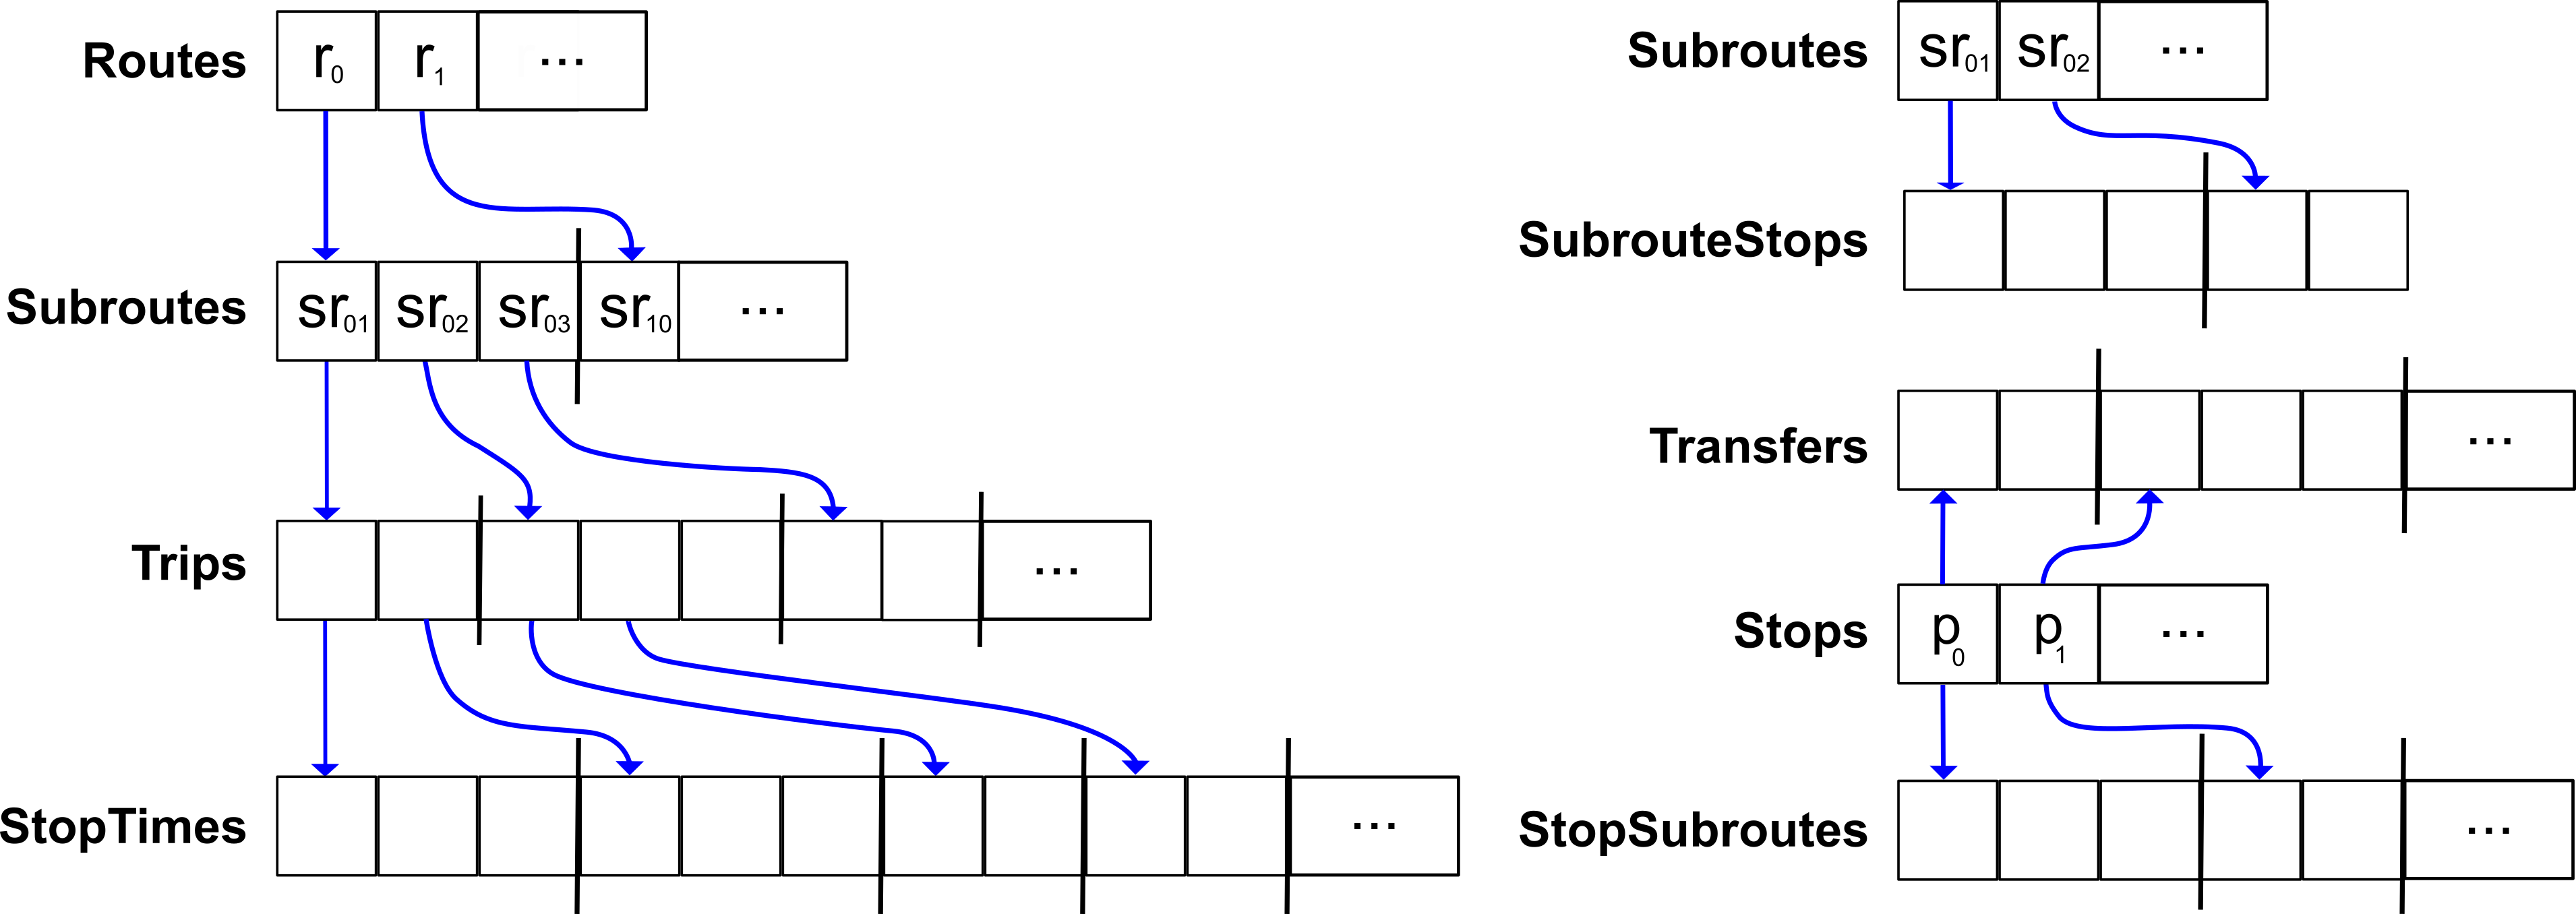
\includegraphics[width=1.0\textwidth]{images/my-structure}}
\caption[Návrh dátovej štruktúry]{Návrh dátovej štruktúry}
\label{fig:my-datastructure}
\end{figure}

V algoritme sa potrebujeme často dopytovať na všetky linky, ktoré stoja na konkrétnej zastávke. Úseky linky pre zastávku vieme jednoducho získať z poľa \textit{StopSubroutes} a hľadanú linku z poľa \textit{Routes}. Pole \textit{SubrouteStops} priraďuje postupnosť zastávok konkrétnemu úseku linky. Zastávky sú zoradené podľa časov príchodu linky na jednotlivé zastávky.

Algoritmus potrebuje často k svojim výpočtom nájsť jazdu linky \textit{t}, ktorá stojí na zastávke \textit{p} najskôr od zadaného času $\tau$ v zadanom type dňa (pracovný deň, víkend, ...). 
Aby sme pri hľadaní jazdy linky nemuseli prechádzať všetky prvky poľa \textit{Trips}, zoskupili sme navyše jednotlivé jazdy v rámci úseku podľa typu dňa.

V poli \textit{StopTimes} nebude prvok obsahovať len informáciu o čase, kedy podľa statického poriadku má stáť jazda linky na zastávke, ale aj informáciu o prípadnom časovom meškaní danej jazdy na zastávku. K tomuto údaju bude algoritmus pristupovať len vtedy, ak používateľ vyhľadáva v aktuálny deň. 

Pole \textit{Transfers} obsahuje pre každú zastávku \textit{p} pole zastávok, ktoré sa nachádzajú v blízkosti zastávky \textit{p} spolu s informáciu o časovej vzdialenosti v minútach. Maximálna vzdialenosť peších presunov je 8 minút. 


\section{Architektúra systému}

Klient sa bude dopytovať na server pre vyhľadanie spojenia. Server spustí výpočet nad dátovou štruktúrou, ktorá má aktuálne cestovné poriadky s informáciou o prípadnom meškaní spojov a vráti odpoveď klientovi.

Algoritmus bude pracovať nad dátovou štruktúrou, ktorá bude obsahovať stále aktuálne dáta. Dátová štruktúra bude rovnako ako algoritmus uložená na serverovej strane. 

\subsection{Serverová strana}
Na serverovej strane bude bežať aplikačný server \textit{Tomcat}. Na uchovanie dát použijeme relačnú databázu. Na komunikáciu s klientom budeme používať \textit{REST API}.

\subsection{Klientská strana}
Na klientskej strane sme sa rozhodli pre progresívnu webovú aplikáciu. Je to webová aplikácia, ktorá sa dokáže správať ako mobilná aplikácia, neustále sa aktualizuje, pričom nie je potrebná jej inštalácia. Po návšteve webovej stránky na mobilnom zariadení používateľ dostane upozornenie od stránky, či si ju chce uložiť do zariadenia ako mobilnú aplikáciu. Progresívna webová aplikácia zaberá minimum miesta v pamäti a má svoj vlastný úložný priestor, kde sa budú ukladať preferencie a história vyhľadávania.

\subsection{Spracovanie dát}
Pri spustení aplikácie alebo po aktualizácii cestovných poriadkov sa spustí služba, ktorá z úložiska, kde sú aktuálne cestovné poriadky namapuje dáta do našej databázy a do dátovej štruktúry. 

Ďalšia služba bude vytvorená na spracovanie údajov o meškaní. Hoci máme v súbore pre konkrétny deň údaje o meškaní jázd na celý deň, chceme sa čo najviac priblížiť reálnemu nasadeniu. Budeme teda počítať s tým, že nové údaje o meškaní pribúdajú po minúte. Služba bude spúšťaná každú minútu. Bude čítať súbor pre aktuálny deň, získa záznamy, ktoré pribudli v poslednej minúte a aktualizuje meškanie pre konkrétne jazdy. Údaje o meškaní sú evidované pre zastávku \textit{p}, na ktorej meškanie vzniklo. Aktualizácia meškania jazdy bude prebiehať tak, že pre všetky zastávky jazdy od zastávky \textit{p} až po konečnú zastávku jazdy zapíše do dátovej štruktúry hodnotu získaného meškania.

Spôsob akým bude aplikácia nasadená je znázornená na obrázku \ref{fig:deploymentDiagram}.

\begin{figure}[H]
\centerline{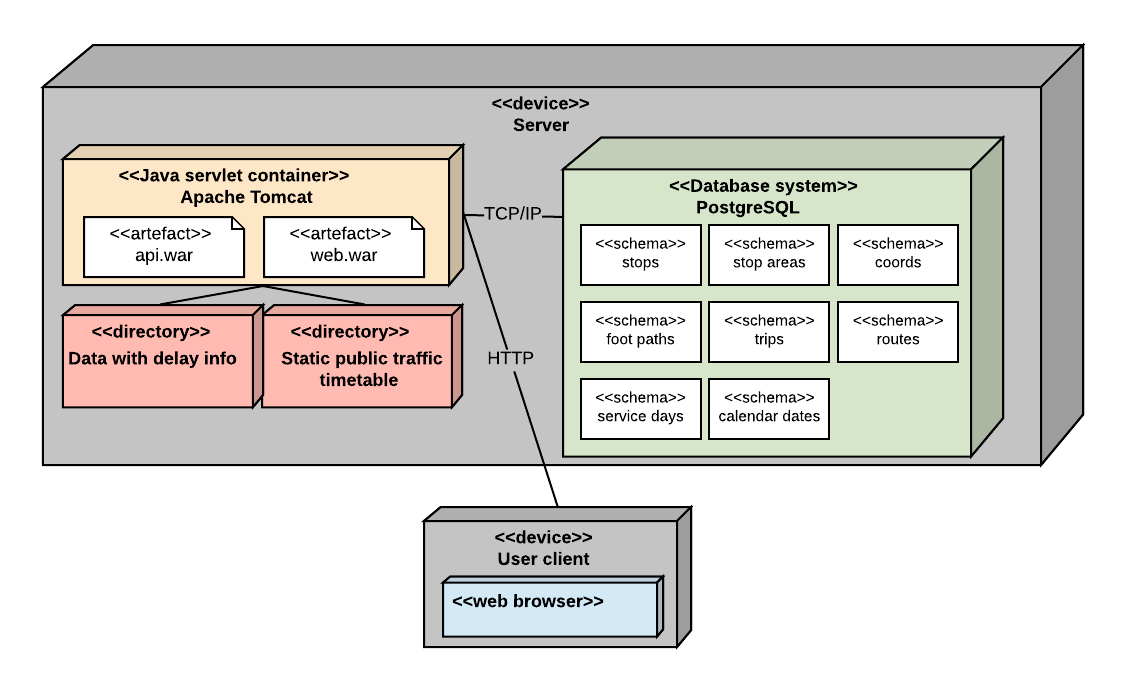
\includegraphics[width=0.8\textwidth]{images/deployment-diagram}}
\caption[Diagram nasadenia]{Diagram nasadenia}
\label{fig:deploymentDiagram}
\end{figure}



